\section{Kernel Discriminant Analysis against Masking}
\subsection{Linear Discriminant Analysis}

%\begin{frame}
%\frametitle{Contents}
%\begin{itemize}
%\item \important{Introduction to LDA: as a classifier, and as a feature extractor}
%\item Introduction to masking countermeasure and Kernel Discriminant Analysis as a feature extractor
%\item Motivations to apply deep learning techniques
%\item Convolutional Neural Networks and Data Augmentation to attack jitter-based countermeasure
%\end{itemize}
%\end{frame}

\begin{frame}{Linear Dimensionality Reduction}
\begin{figure}
\centering{
\resizebox{11cm}{!}
{
\begin{tikzpicture}[remember picture,
    scale=0.50,
    % Define styles here
    every node/.style={transform shape}
    block/.style={
        rectangle,
        draw,
        text centered,
        rounded corners
        },
    data/.style={
        trapezium,
        trapezium left angle=60,
        trapezium right angle=120,
        draw
        },
    component/.style={
        circle,
        draw
        },
    output/.style={
        tape,
        tape bend top=none,
        draw
        },
    edge/.style={
        ->,
        >=stealth,
        thick
        }
    ]

    % Place nodes
    \node[inner sep=0pt] (genericTrace) at (0,-0)
    {\includegraphics[width=0.8\textwidth]{figures/genericTrace.pdf} };
    \node [above=0.1cm of genericTrace] {Rough Trace};
    \node [block, below left=0.8cm of genericTrace] (PCA) {\begin{Large}PCA\end{Large}};
    \node [block, below right=0.8cm of genericTrace] (LDA) {\begin{Large}LDA\end{Large}};
    \node [below=1.5cm of genericTrace](puntini) {\begin{Large}$\dots$\end{Large}};
    \node [component, left=0.5cm of puntini](PC2) {\begin{Large}$\AAlpha_2$\end{Large}};
    \node [component, left=0.5cm of PC2](PC1) {\begin{Large}$\AAlpha_1$\end{Large}};
    \node [component, right=0.25cm of puntini](PCC) {\begin{Large}$\AAlpha_C$\end{Large}};
   \node [right=0.25cm of PCC](puntini2) {\begin{Large}$\dots$\end{Large}};
    \node [component, right=0.15cm of puntini2](PCr) {\begin{Large}$\AAlpha_r$\end{Large}};
    %\draw[thick, black,decorate,decoration={brace,amplitude=10pt}](PC1.north) -- (PCr.north);
    \draw(PC1.north)  to [bend left=15] (PCr.north);
    
    
    \draw[->, shorten >=20pt] (PCA.north) node[above=0.4cm] {Principal Components (PCs)} to [bend left] (PC2.north) ;
     \draw[->,shorten >=25pt] (LDA.north)  node[above=0.35cm] {Discriminant Components (DCs)} to [bend right] (puntini2.north);
     
    \only<2>{ 
    \node [data, below=1cm of puntini](formula1) {\begin{Large}$\sum_{j=1}^D\AAlpha_1[j]\textbf{x}[j]$\end{Large}};
    \node [left=0.5cm of formula1] {Linear Combination / Projection};
    \node [below=0.5cm of formula1] (compressed1)
    	{\includegraphics[width=0.5\textwidth]{figures/compressed1.pdf} }; 
    	\node[right=0.1cm of compressed1]{Reduced Trace}; 
	\draw[-, red, thick, shorten >=6pt, shorten <=-6pt](genericTrace.south) to (PC1.north);
	\draw[-, red, thick, shorten >=6pt, shorten <= 6pt](PC1.south) to (formula1.north);
	\draw[-, red, thick, shorten <= 2pt, shorten >=-5pt](formula1.south) to (compressed1.north);
}
    
        \only<3>{ 
        \node [data, below=1cm of puntini](formula2) {\begin{Large}$\sum_{j=1}^D\AAlpha_2[j]\textbf{x}				[j]$\end{Large}};
    \node [left=0.5cm of formula2] {Linear Combination / Projection};
    \node [below=0.5cm of formula2] (compressed2)
    	{\includegraphics[width=0.5\textwidth]{figures/compressed2.pdf} };  
    	\node[right=0.1cm of compressed2]{Reduced Trace};
	\draw[-, red, thick, shorten >=6pt, shorten <=-6pt](genericTrace.south) to (PC2.north);
	\draw[-, red, thick, shorten >=6pt, shorten <= 6pt](PC2.south) to (formula1.north);
	\draw[-, red, thick, shorten <= 2pt, shorten >=-5pt](formula2.south) to (compressed2.north);
}

 \uncover<4>{ 
        \node [data, below=1cm of puntini](formulaC) {\begin{Large}$\sum_{j=1}^D\AAlpha_C[j]\textbf{x}				[j]$\end{Large}};
    \node [left=0.5cm of formulaC] {Linear Combination / Projection};
    \node [below=0.5cm of formulaC] (compressedC)
    	{\includegraphics[width=0.5\textwidth]{figures/compressedAll.pdf} }; 
    \node[right=0.1cm of compressedC]{Reduced Trace};
	\draw[-, red, thick, shorten >=6pt, shorten <=-6pt](genericTrace.south) to (PCC.north);
	\draw[-, red, thick, shorten >=6pt, shorten <= 6pt](PCC.south) to (formulaC.north);
	\draw[-, red, thick, shorten <= 2pt, shorten >=-5pt](formulaC.south) to (compressedC.north);
}
    
     
     

\end{tikzpicture}
}
}

\end{figure}
\end{frame}

\begin{frame}
\frametitle{Model-based SNR and Fisher's Criterion}
\begin{block}{Signal-to-Noise Ratio (SNR)}
\begin{itemize}
\item Independent Noise Assumption: $\vaLeakVec = \varphi(\sensRandVar)+\vec{B}$

\item $\mmmXclass= \esperEst[\given{\vaLeakVec}{\sensRandVar = \sensVarGenValue}] = \frac{1}{\nbTracesPerClass}\sum_{i\colon \sensVar_i=\sensVarGenValue} \vLeakVec_i $ sample mean per class ($\approx \varphi(\sensRandVar)$)
\item $\varXclass = \varEst(\given{\vaLeakVec}{\sensRandVar = \sensVarGenValue}) = \frac{1}{\nbTracesPerClass-1}\sum_{i\colon \sensVar_i=\sensVarGenValue} (\vLeakVec_i - \mmmXclass)^2 $ sample variance per class ($\approx \mathrm{var}(\vec{B})$) 
\item \begin{equation*}\mathrm{SNR}(t) = \frac{\varEst(\mmmXclass[Z](t))}{\esperEst[\varXclass[Z](t)]} \qquad \textcolor{grey}{\frac{\text{\emph{variance inter-class}}}{\text{\emph{variance intra-class}}}} \end{equation*}
\end{itemize}
\end{block}

\begin{block}{Fisher's Criterion for Linear Dimensionality Reduction}

\begin{itemize}
\item $\SB = \sum_{\sensVarGenValue\in\sensVarSet}\nbTracesPerClass(\mmmXclass-\mmmX)(\mmmXclass-\mmmX)^\intercal $ (inter-class scatter matrix)
\item $\SW = \sum_{\sensVarGenValue\in\sensVarSet}\sum_{i=1\colon \sensVar_i=\sensVarGenValue}(\vLeakVec_i-\mmmXclass)(\vLeakVec_i-\mmmXclass)^\intercal$ (intra-class scatter matrix)
\item Fisher's criterion
 \begin{equation}\label{eq:LDA}
\hat{ \AAlpha}=\mathrm{argmax}_{\AAlpha} \frac{\AAlpha^\intercal \SB \AAlpha}{\AAlpha^\intercal \SW \AAlpha} \mbox{ ,}
 \end{equation}
\end{itemize}

\end{block}
\end{frame}

\begin{frame}
\frametitle{LDA: an optimal binary linear classifier}
\begin{columns}
\begin{column}{.5\linewidth}
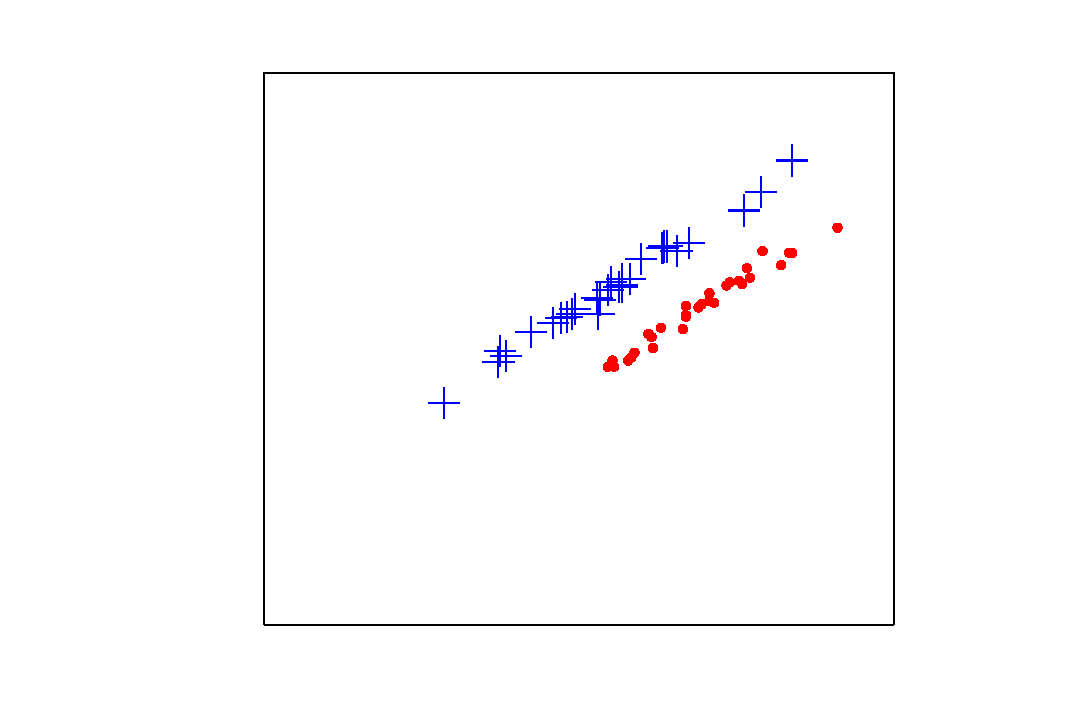
\includegraphics[width=\textwidth]{figures/dataNoProjection.pdf} 
\end{column}
\begin{column}{.6\linewidth}
\begin{itemize}
\item Classify data $\vLeakVec$ into 2 classes $\sensVarSet = \{\sensVarValue{1}, \sensVarValue{2}\}$
\item Generative model: $\pdf_{\given{\vaLeakVec}{\sensRandVar = \sensVarValue{j}}}(\vLeakVec)$, $\pdf_{\sensRandVar}(\sensVarValue{j})$ and $\pdf_{\vaLeakVec}(\vLeakVec)$
\item Posterior probabilities (via Bayes' theorem), then classify through the \emph{log-likelihood ratio}: $a = \log\left[\frac{\prob(\given{\sensVarValue{1}}{\vLeakVec})}{\prob(\given{\sensVarValue{2}}{\vLeakVec})}\right]]$ (boundary surface $a=0$)
\end{itemize}
\end{column}
\end{columns}

\begin{itemize}
\item Two assumptions about class-conditional densities: 
\begin{itemize}
\item Gaussian distributions with parameters $\mu_j, \Sigma_j$
\item Homoscedasticity: $\Sigma_j=\Sigma$ for all $j$
\end{itemize}
\item $\Rightarrow a = \vec{w}^\intercal \vLeakVec + w_0$ (linear decision boundary, $\vec{w}$ and $w_0$ functions of $\Sigma, \mu_j$)
\end{itemize}

\end{frame}

\begin{frame}
\frametitle{LDA and Fisher's Discriminant}
\begin{columns}
\begin{column}{.5\linewidth}
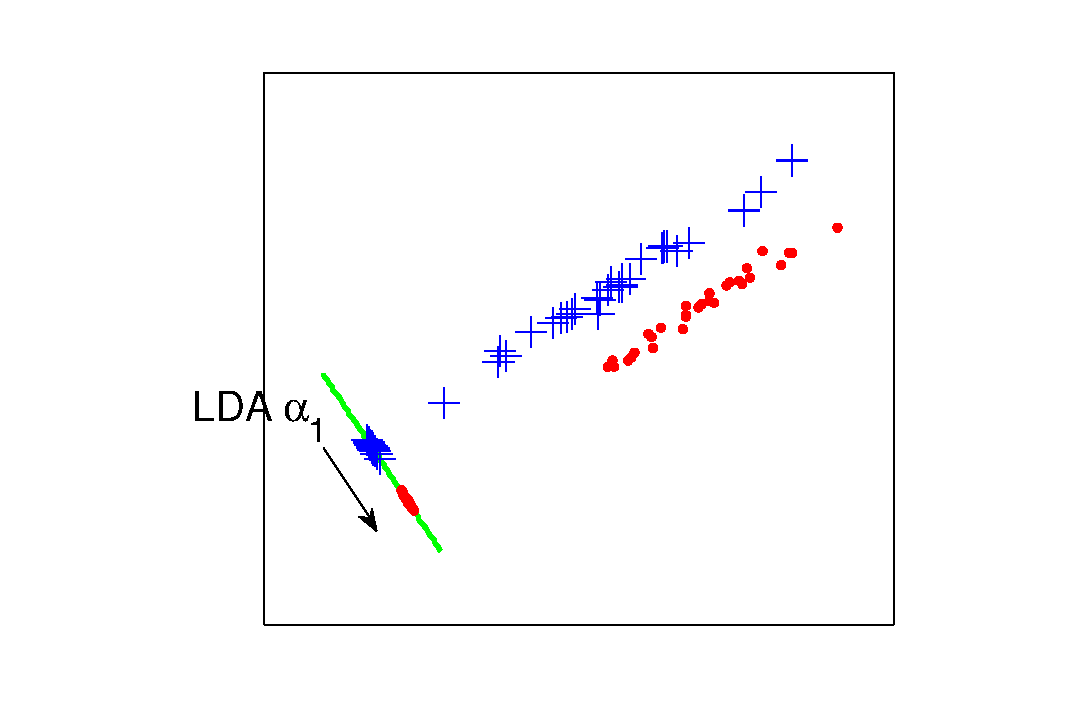
\includegraphics[width=\textwidth]{figures/LDAprojection.pdf} 
\end{column}
\begin{column}{.6\linewidth}
\begin{itemize}
\item LDA: linear decision boundary $a = \vec{w}^\intercal \vLeakVec + w_0$
\item Equivalently, project data onto $\vec{w}^\intercal \vLeakVec$ (orthogonally to the decision boudary), than classify by a real threshold (optimally $w_0$). \\
\end{itemize}
\end{column}
\end{columns}

\begin{itemize}
\item Two assumptions about class-conditional densities: 
\begin{itemize}
\item Gaussian distributions with parameters $\mu_j, \Sigma_j$
\item Homoscedasticity: $\Sigma_j=\Sigma$ for all $j$
\end{itemize}
\end{itemize}

\begin{block}{Fact, abuse and preference for the dimensionality reduction formulation}
\begin{itemize}
\item When LDA assumptions are met, the solution of the Fisher's criterion coincides with $\vec{w}$. 
\item assumption not required
\item naturally multi-class
\end{itemize}
\end{block}

\end{frame}

\begin{frame}
\frametitle{Linear separability}
LDA: linear decision boundary $a = \vec{w}^\intercal \vLeakVec + w_0$ ($\vec{w} = \Sigma^{-1}(\mu_1-\mu_2)$)
%
\begin{block}{}
\begin{huge}
If $\mu_1 = \mu_2$? 
\end{huge}
\end{block}
\end{frame}

\begin{frame}
\frametitle{Dimensionality reduction in presence of sharing}
%\begin{block}{Countermeasures}
%Techniques to thwart side-channel attacks. 
%\begin{itemize}
%\item Hiding (\emph{ex:} random delay, shuffling, ...)
%\item Sharing  $\textcolor{red}{\longleftarrow}$ \textcolor{red}{makes selecting and projecting techniques ineffective}
%\end{itemize}
%\end{block}


\begin{block}{$(d-1)$th-order Sharing (or Masking)}
$Z$ split into shares  $Z = M_1 \star \dots \star M_d$ \\
with $M_1, \dots , M_{d-1}$ random shares (or masks) and $M_d = Z \star M_1^{-1}\star \dots \star M_{d-1}^{-1}$ \\
Shares are handled at different time samples $t_1,\dots, t_d$ so that each time sample is independent from $Z$: $f(Z) = \esper[\vaLeakVec\lvert Z]$ is constant.
\end{block}
\pause
\begin{block}{Higher-Order SCAs}
Exploit $f(Z) = \esper[\vaLeakVec[t_1]\vaLeakVec[t_2]\dots\vaLeakVec[t_d]\lvert Z]$ non-constant.\\
 
The statistic extracted from measurements, viewed as a multivariate polynomial in the time samples coordinates, must contain the $d$th-degree monomial $\vaLeakVec[t_1]\vaLeakVec[t_2]\dots\vaLeakVec[t_d]$.
\end{block}

\end{frame}

\begin{frame}
\frametitle{PoIs Research}
How to detect the $d$-tuple $t_1,\dots, t_d$? 
\begin{block}{A lacking literature}
\begin{itemize}
\item many HO attacks papers assume the knowledge of $t_1,\dots, t_d$
\item PoI research exploiting the random shares knowledge (back to unprotected case using $M_1,\dots , M_d$ instead of $Z$)
\item naive strategy: infer over all possible $d$-tuples 
\item Hand selection via educated guess \cite{Oswald2006}
\end{itemize}
\end{block}

\begin{block}{Generalizing extractors for higher-order context}
\begin{itemize}
\item Selecting extractors $\longrightarrow$ Projection Pursuits \cite{PP}
\item Projecting extractors $\longrightarrow$ Kernel Discriminant Analysis [CARDIS '16]
\end{itemize}
\end{block}
\end{frame}

\subsection{Kernel Discriminant Analysis}
\begin{frame}
[fragile]
\frametitle{Kernel Discriminant Analysis (KDA) [to appear at CARDIS '16]}
\vspace{-10pt}
\begin{figure}
\centering
{
\begin{tikzpicture}
\matrix (m) [matrix of math nodes, row sep=3em,
column sep=3em, text height=1.5ex, text depth=0.25ex]
{ \mathbb{R}^\traceLength & \featureSpace & \mathbb{R}^\newTraceLength \\ };
\path[->]
(m-1-1) edge node[above] {$\Phi$} (m-1-2);
         %edge [bend left=30] (m-2-2)
         %edge [bend right=15] (m-2-2);
\path[->]
($(m-1-2.north east)-(0,0.1)$) edge node[above] {$\extract^{\mathrm{PCA}}$} ($(m-1-3.north west)-(0,0.1)$);
\path[->]
($(m-1-2.south east)+(0,0.15)$) edge node[below] {$\extract^{\mathrm{LDA}}$} ($(m-1-3.south west)+(0,0.15)$);

\path[->]
(m-1-1) edge [bend left=50] node[above] {$\extract^{\mathrm{KPCA}}$} (m-1-3)
(m-1-1) edge [bend right=50] node[below] {$\extract^{\mathrm{KDA}}$} (m-1-3);

\end{tikzpicture} 
}
\end{figure}
\vspace{-10pt}
$\mathcal{F}$ contains all $d$-th degree monomials \small{(dimension increases combinatorially: ${{D}\choose{d}}$)}
\pause

\begin{block}{Kernel function}
 \begin{centering}$K\colon\mathbb{R}^D\times \mathbb{R}^D \rightarrow \mathbb{R} \qquad K(\vLeakVec[]{i},\vLeakVec[]{j}) = \Phi(\vLeakVec[]{i})\cdot \Phi(\vLeakVec[]{j})
$\end{centering}
\end{block}
\pause
\vspace{-5pt}
\begin{block}{Polynomial kernel function}
dth-degree polynomial kernel: $K\colon(\vLeakVec[]{i},\vLeakVec[]{j}) \mapsto ( \vLeakVec[]{i}\cdot \vLeakVec[]{j})^d \leftrightarrow$  all $d$-th degree monomials ($\mathcal{F}$).
\pause

Example: 
$d=2, D=2$; $\vLeakVec[]{i} = [a,b]$ , $\vLeakVec[]{j} = [c,d]$ $\longrightarrow$
\vspace{-10pt}
\begin{equation*}
\textcolor{olive}{K(\vLeakVec[]{i},\vLeakVec[]{j})} = (ac + bd)^2 = a^2c^2 + 2abcd + b^2d^2 \mbox{ ,}
\end{equation*}

%\begin{align}
%&\Phi \colon \mathbb{R}^2 \rightarrow \mathbb{R}^3\\
%&\Phi \colon [a,b]\mapsto [a^2, \sqrt{2}ab, b^2]\\
%&\Phi \colon [c,d]\mapsto [c^2, \sqrt{2}cd, d^2].
%\end{align}
\vspace{-15pt}
\begin{equation*}
K \longleftrightarrow \Phi\colon \Bbb{R}^2\rightarrow\Bbb{R}^3 \qquad \Phi(u,v) =  [u^2, \sqrt{2}uv, v^2]
\end{equation*}
$\textcolor{olive}{\Phi(\vLeakVec[]{i})\cdot \Phi(\vLeakVec[]{j})} = a^2c^2 + 2abcd + b^2d^2 = K(\vLeakVec[]{i},\vLeakVec[]{j})$

\end{block}
\end{frame}

\begin{frame}
[fragile]
\frametitle{LDA to KDA}
\vspace{-30pt}
\begin{figure}
\centering
{
\begin{tikzpicture}
\matrix (m) [matrix of math nodes, row sep=3em,
column sep=3em, text height=1.5ex, text depth=0.25ex]
{ \mathbb{R}^\traceLength & \featureSpace & \mathbb{R}^\newTraceLength \\ };
\path[->]
(m-1-1) edge node[above] {$\Phi$} (m-1-2);
         %edge [bend left=30] (m-2-2)
         %edge [bend right=15] (m-2-2);
\path[->]
($(m-1-2.north east)-(0,0.1)$) edge node[above] {$\extract^{\mathrm{PCA}}$} ($(m-1-3.north west)-(0,0.1)$);
\path[->]
($(m-1-2.south east)+(0,0.15)$) edge node[below] {$\extract^{\mathrm{LDA}}$} ($(m-1-3.south west)+(0,0.15)$);

\path[->]
(m-1-1) edge [bend left=50] node[above] {$\extract^{\mathrm{KPCA}}$} (m-1-3)
(m-1-1) edge [bend right=50] node[below] {$\extract^{\mathrm{KDA}}$} (m-1-3);

\end{tikzpicture} 
}
\end{figure}
\vspace{-15pt}
\begin{columns}
\begin{column}{.5\textwidth}
\begin{block}{LDA}
\begin{itemize}
\item $\AAlpha_i$ eigenvectors of $\SW^{-1}\SB$
\item $\SB$ and $\SW$ depend on data $(\vLeakVec[z_i]{i})$ [$D\times D$]
\item $\extract^{LDA}_{\ell}(\vaLeakVec) = \sum_{i=1}^D \AAlpha_{\ell}[i]\vaLeakVec[i] $
\end{itemize}
\end{block}
\end{column}

\begin{column}{.5\textwidth}
\begin{block}{KDA}
\begin{itemize}
\item $\nununu_i$ eigenvectors of $(\SW^K)^{-1}\SB^K$
\item $\SB^K$ and $\SW^K$ depend on kernel function images $K(\vLeakVec[z_i]{i}, \vLeakVec[z_j]{j})$ [$N\times N$]
\item $\extract^{\mathrm{KDA}}_{\ell}(\vec{x}) = \sum_{i=1}^{\numPoI}\nununu_\ell[i]K(\vLeakVec[z_i]{i}, \vLeakVec[]{}) $
\end{itemize}
\end{block}
\end{column}
\end{columns}
\vspace{-5pt}
\begin{block}{Application Issues}
\begin{itemize}
\item regularization : $\SW^K \leftarrow \SW^K + \mu \III$
\item computational complexity is $O(N^3)$ 
\item non-injective model $\sensVarSet \rightarrow m(\sensVarSet)$ to reduce the number of classes (to improve KDA accuracy in detecting class separating subspaces)
\item asymmetric 'KDA/profiling' approach (to improve profiling accuracy)
\end{itemize}
\end{block}

\end{frame}

\subsection{Experimental Results}


\begin{frame}
\frametitle{Experimental results}
\begin{itemize}
\item $D = 200$: length of rough trace (interesting clock cycles selected)
\item $d=2$, feature extracted from a $200^2 = 40.000$-sized space
\item $d=3 \rightarrow 200^3=6.000.000$ , $d=4 \rightarrow 200^4 = 800.000.000$
\end{itemize}
\begin{figure}[t]

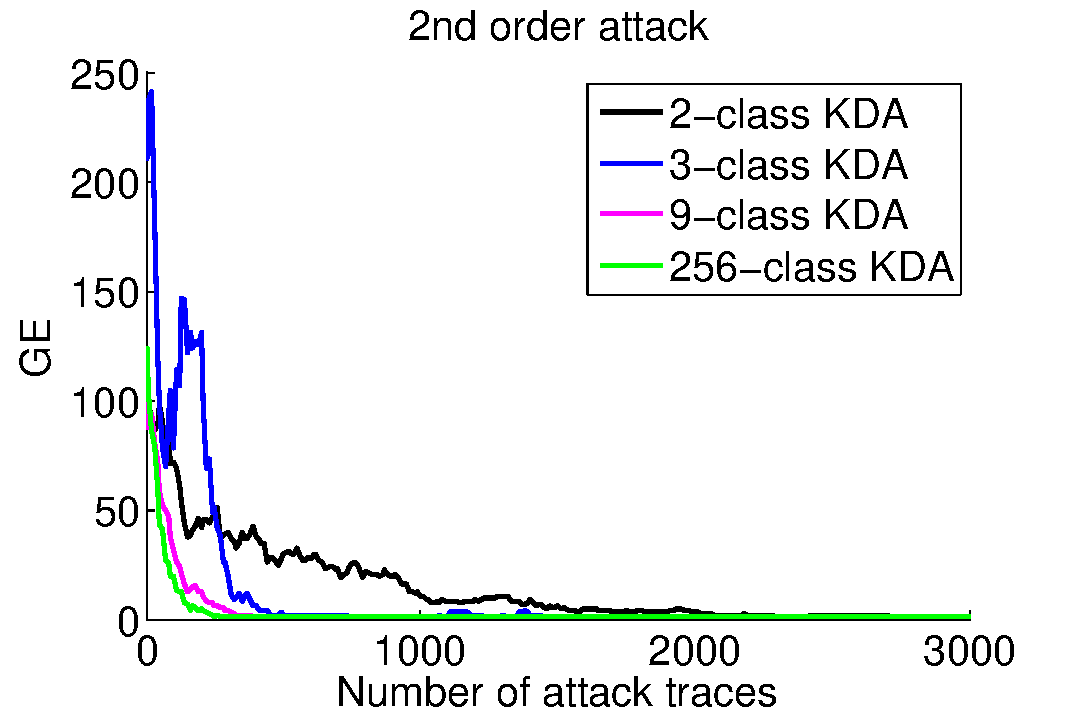
\includegraphics[width=.4\textwidth]{../Figures/CARDIS2016/2order_classes_TA.pdf}
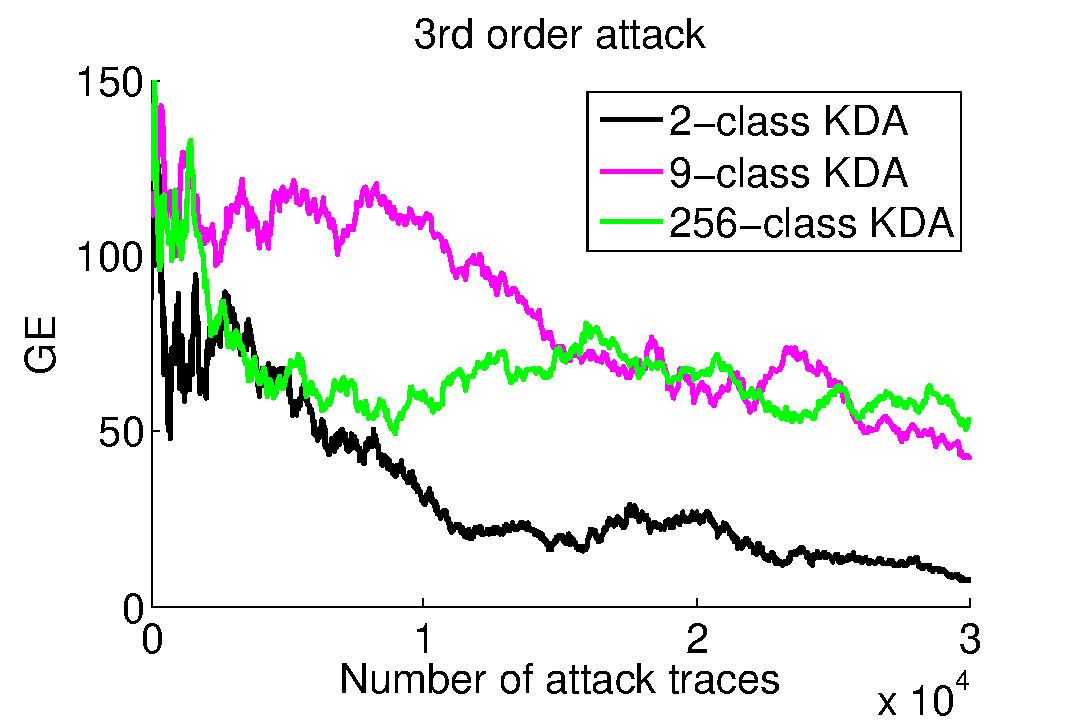
\includegraphics[width=.4\textwidth]{../Figures/CARDIS2016/3order_new.pdf}
\end{figure}
\vspace{-10pt}
\begin{figure}[t]

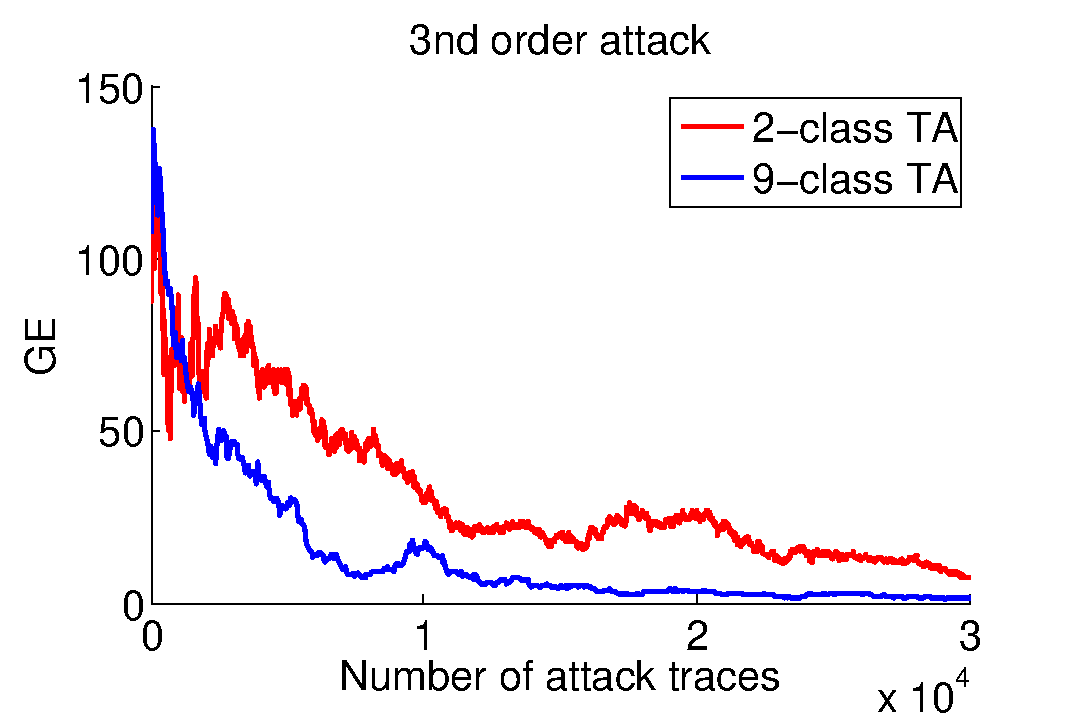
\includegraphics[width=.4\textwidth]{../Figures/CARDIS2016/3order_2_9.pdf}
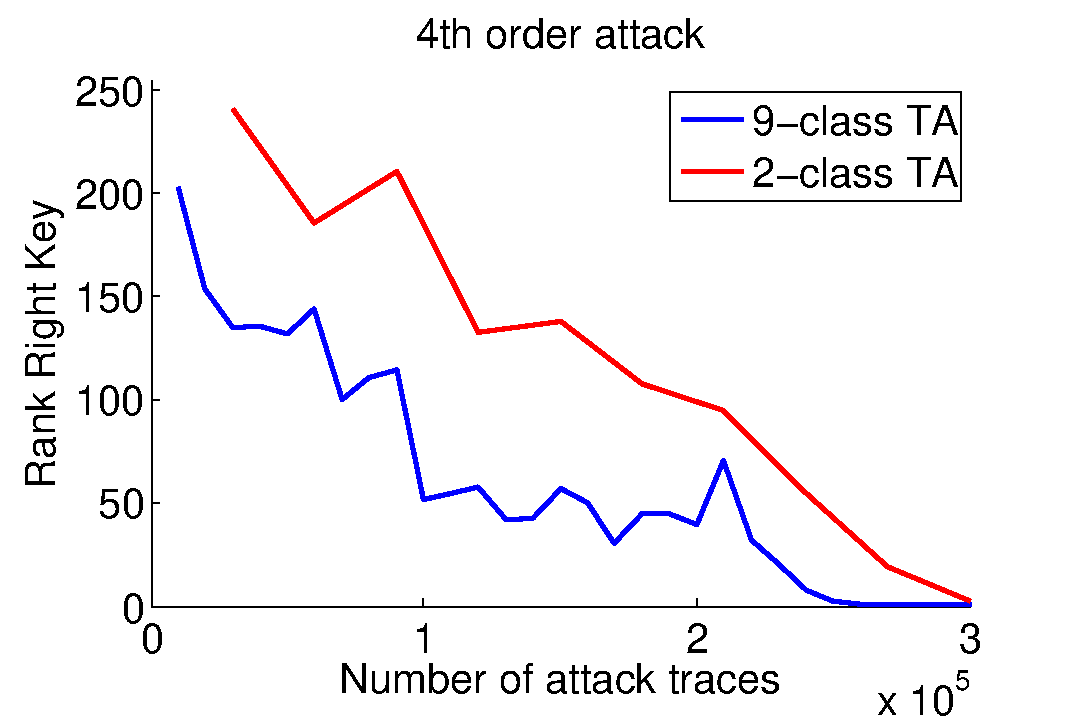
\includegraphics[width=.4\textwidth]{../Figures/CARDIS2016/4order_2_9.pdf}
\end{figure}
\end{frame}

\begin{frame}
\frametitle{Limits and Drawbacks}

\end{frame}